\documentclass{article}
\usepackage[dblblindworkshop]{neurips_2026}
\workshoptitle{TAE (Trust-AI-Eval): Can We Trust AI Evaluation?}

\usepackage[utf8]{inputenc}
\usepackage[T1]{fontenc}
\usepackage{hyperref}
\usepackage{url}
\usepackage{booktabs}
\usepackage{amsfonts}
\usepackage{amsmath}
\usepackage{nicefrac}
\usepackage{microtype}
\usepackage{graphicx}

\title{Measure the instrument first:\\detection floors for model-selection pipelines}

\author{Anonymous Author(s)\\Affiliation\\Address\\\texttt{email}}

\begin{document}
\maketitle

\begin{abstract}
A selection pipeline reports that a candidate improved a metric. It almost never reports the smallest improvement it could have detected, and those are different claims. We measure the second one on a deployed forecasting system using a construction that needs no assumptions: the \emph{null lever} --- the same recipe refit under a different random seed --- changes nothing real, so everything it produces is instrument noise. On a $4{,}141$-row walk-forward pool scored under five seeds, ten such comparisons give a one-sided $80\%$ detection floor of $0.00307$ nats, and the largest effect a null lever manufactured is $0.00230$ nats. The only lever this system ever shipped is worth $0.0026$: re-seeding alone reproduces $88\%$ of it. Two consequences generalise beyond the case. First, \textbf{buying seeds cannot fix an underpowered arm}: $54\%$ of the variance is row-level and immune to seed budget, so an infinite budget moves the floor by $1.36\times$ and no further. Second, \textbf{the floor is a property of the question count, not just the data}: the same pipeline asking $84$ pre-registered questions has a floor of $0.00505$, above every candidate it evaluated. We give the protocol, a decomposition that says which purchase would help, and a documented case of a selection split choosing the worst of six candidates because it sat below its own floor.
\end{abstract}

\section{The number that is missing from the report}

Evaluation reports are asymmetric. They state what changed and by how much; they rarely state what the pipeline could have resolved. When the second number is absent a reader cannot distinguish three situations that demand different responses --- a real improvement, a real improvement too small to have been seen, and noise --- and in our experience the third is the most common and the least often named.

This is not a call for more error bars. Error bars on a single arm do not answer the question, because the quantity a candidate must clear is not the spread of the metric but the spread of the \emph{difference} under a change that does nothing. That quantity is directly measurable, and measuring it is cheap.

We report it for a deployed sports-outcome forecasting system whose model-selection pipeline has been in continuous use for roughly a year, has evaluated several dozen candidate levers, and has shipped exactly one. The system is a gradient-boosted ensemble over $118$ point-in-time features; selection runs on a walk-forward out-of-fold pool built from $32$ quarterly refits, so a candidate is scored only on rows no fold of it was trained on. None of that matters to the argument. What matters is that the pipeline is stochastic, that it was run five times under five seeds, and that those five runs are enough to say what it can see.

\textbf{Contributions.} (i) A protocol --- the null lever --- for measuring a selection instrument's detection floor with no distributional assumption and no extra experiments beyond re-seeding. (ii) A variance decomposition that says which purchase raises power, and the finding that the usual purchase does not: seed budget addresses under half the variance and saturates within about five seeds. (iii) A quantification of what asking more questions does to the floor, on the same pipeline. (iv) A documented failure --- a selection split, below its own floor, choosing the worst of six candidates --- and the multi-basis discipline that replaced it.

\textbf{Related work.} That benchmark conclusions are unstable under nuisance variation is well established: \citet{dodge2019} showed reported results depend on search budget and asked for it to be published; \citet{bouthillier2021} decomposed benchmark variance into its sources and argued for randomising more of them; \citet{card2020} computed statistical power for NLP experiments and found much of the literature underpowered; \citet{gorman2019} showed that conclusions drawn on a standard split often fail to hold on random ones. Our contribution is not the observation but the operational form. Those works estimate variance in order to argue that reported effects may be noise; we invert it into a single number a pipeline can print next to each decision --- the largest effect a change that does nothing was able to manufacture --- and then ask which purchase, seeds or rows, would move it. The multiplicity term in Section~6 is the same charge \citet{by2001} formalise for testing, applied to selection, where it is usually not charged at all.

\section{The null lever}

Let a \emph{lever} be any change to a recipe that a pipeline may accept or reject, and let $\widehat\Delta$ be the paired difference in the selection metric between the levered and unlevered arms on the same evaluation rows. A \emph{null lever} is a change that alters no modelling decision --- here, the random seed passed to the learners.

Under a null lever $\mathbb{E}[\widehat\Delta]=0$ by construction. Its realised distribution is therefore the pipeline's noise distribution, measured rather than modelled, and the smallest real effect the pipeline can distinguish from that noise is
\begin{equation}
\mathrm{MDE} \;=\; \big(z_{1-\alpha} + z_{\mathrm{power}}\big)\cdot \mathrm{SE}(\widehat\Delta),
\end{equation}
with $\mathrm{SE}$ estimated from the null lever itself. Five seeds give $\binom{5}{2}=10$ null comparisons at no cost beyond the reruns a careful project already performs.

Two properties make this preferable to the alternatives. It requires no assumption about the metric's sampling distribution, because it draws from the real one. And it is \emph{paired on evaluation rows}, which removes the shared difficulty of the examples --- the dominant term in any absolute metric, and the term that makes single-arm error bars look reassuring while telling you nothing about the comparison you are actually making.

\section{What the instrument can see}

\begin{table}[t]
\centering\small
\begin{tabular}{lr}
\toprule
quantity & value \\
\midrule
evaluation rows (walk-forward, out-of-fold) & $4{,}141$ \\
per-seed metric, five seeds & $0.64142$ -- $0.64372$ \\
sd of the metric across seeds & $0.00086$ \\
\midrule
null-lever comparisons & $10$ \\
paired SE of a null lever & $0.00091$ \\
\textbf{largest effect a null lever manufactured} & $\mathbf{0.00230}$ \\
\midrule
variance that is row-level (no seed budget touches it) & $54\%$ \\
variance that is seed-level & $46\%$ \\
\midrule
detection floor, one seed & $0.00307$ \\
detection floor, infinite seeds & $0.00226$ \\
detection floor, one seed, $84$ questions & $0.00505$ \\
\midrule
\textbf{the only lever this system ever shipped} & $\mathbf{0.0026}$ \\
\bottomrule
\end{tabular}
\caption{The instrument, and the one candidate that survived it. Metric is out-of-fold log-loss; lower is better; floors are one-sided at $\alpha=0.05$ and $80\%$ power.}
\label{tab:floor}
\end{table}

Table~\ref{tab:floor} is the whole measurement. The line that should be read first is not the floor but the one above it: \textbf{the largest difference produced by a change that did nothing is $0.00230$ nats}, and the only improvement this system has ever shipped is worth $0.0026$. Re-seeding reproduces $88\%$ of the project's single genuine result. Had that lever been evaluated once, under one seed, against one baseline, its measured effect would have been indistinguishable from a rerun.

We note a coincidence that is not one: the empirical maximum over ten null comparisons ($0.00230$) lands almost exactly on the asymptotic floor computed from the variance decomposition ($0.00226$). The two estimates are constructed differently and agree, which is the cheapest available check that the decomposition in the next section is not an artefact of it.

\section{Buying seeds walks to a floor, not past it}

\begin{figure}[t]
\centering
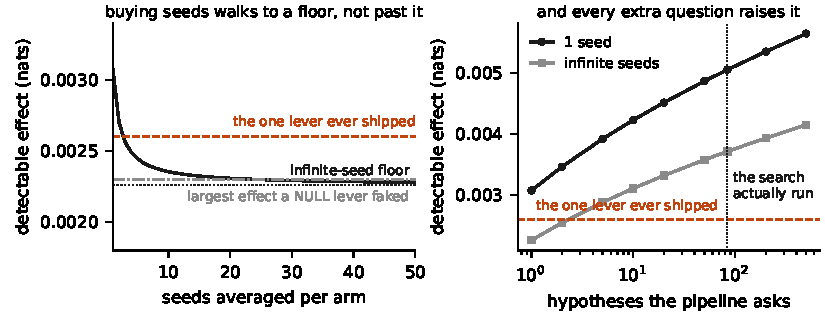
\includegraphics[width=\textwidth]{figs/floor.pdf}
\caption{Left: the detection floor against the number of seeds averaged per arm. The curve saturates within about five seeds because most of the variance is not seed variance. Right: the floor against the number of hypotheses the pipeline asks, at one seed and at an infinite seed budget. The one lever the system ever shipped is below almost every point on both panels.}
\label{fig:floor}
\end{figure}

The standard response to a noisy pipeline is to average more seeds. Decomposing the null lever's variance says how much that helps. Writing $\sigma^2_{\text{row}}$ for the component that comes from which rows the pool happens to contain and $\sigma^2_{\text{seed}}$ for training stochasticity, averaging $k$ seeds per arm gives
\begin{equation}
\mathrm{SE}_k \;=\; \sqrt{\sigma^2_{\text{row}} + \sigma^2_{\text{seed}}/k}\,,
\end{equation}
which has a horizontal asymptote at $\sqrt{\sigma^2_{\text{row}}}$. On this pipeline $\sigma^2_{\text{row}} = 8.27\times10^{-7}$ and $\sigma^2_{\text{seed}} = 7.02\times10^{-7}$: \textbf{$54\%$ of the variance is untouchable by any seed budget}. The floor falls from $0.00307$ at one seed to $0.00226$ at infinitely many --- a factor of $1.36$ --- and is within $2\%$ of its asymptote by five seeds (Figure~\ref{fig:floor}, left).

The practical reading is a budgeting rule. If a candidate's expected effect is below the asymptote, no number of reruns will make it visible and the only purchases that help are more evaluation rows or a lower-variance metric. If it is between the asymptote and the one-seed floor, a handful of seeds is exactly the right purchase and a large number is waste. A project that does not know which regime it is in will buy seeds in both, and in the first regime it will buy them forever.

\section{Every question the pipeline asks raises the floor}

A detection floor is usually quoted as though it were a property of the dataset. It is a property of the dataset \emph{and} the number of questions put to it. A pipeline that evaluates one pre-specified candidate and one that searches eighty-four are not the same instrument, and the difference is large enough to change verdicts.

The same system ran a pre-registered search of $84$ hypotheses over a related pool. Charging that multiplicity at $\alpha=0.05$ raises the per-test critical value from $1.645$ to $3.241$ and the floor from $0.00307$ to $0.00505$ nats --- a factor of $1.64$, on top of everything in the previous section (Figure~\ref{fig:floor}, right). At $84$ questions the floor sits above \emph{every} candidate this system has ever evaluated, including the one it shipped.

This is the number most often missing from a leaderboard or an ablation table. An ablation with twelve rows is a twelve-hypothesis search whether or not it is described as one, and quoting a floor computed for a single comparison overstates what the table can support by roughly a third. The correction is arithmetic and costs nothing; not making it is a choice about what the reader is allowed to conclude.

\section{What happens when the instrument sits below its own floor}

Before the walk-forward pool existed, this system selected on a held-out split of $429$ rows. A calibration study fit six transform families on that split and read its argmin:

\begin{center}\small
\begin{tabular}{lccc}
\toprule
family (parameters) & selection metric & test metric & selection is right \\
\midrule
identity (0) & $0.6203$ & $0.6198$ & --- \\
temperature (1) & $0.6171$ & $\mathbf{0.6165}$ & $89.6\%$ \\
cubic (2) & $0.6170$ & $0.6173$ & $55.0\%$ \\
beta (2) & $0.6164$ & $0.6181$ & --- \\
beta$_{c_0}$ (2) & $0.6166$ & $0.6171$ & $61.6\%$ \\
\textbf{piecewise (3)} --- \emph{selected} & $\mathbf{0.6163}$ & $0.6193$ & $36.5\%$ \\
\bottomrule
\end{tabular}
\end{center}

The split selected the piecewise family, which is the worst of the five non-trivial candidates on test and barely better than doing nothing. The last column --- resampling the selection split, refitting, and re-scoring the same test set --- shows this was not bad luck: at one parameter the selection is right $89.6\%$ of the time, at two it is a coin flip, and at three it is worse than not selecting at all.

We stress what this case is evidence for. It is not that the candidates were bad, nor that the metric was wrong. Every arm here is a legitimate calibrator and the metric is the deployed one. The failure is that a $429$-row split cannot resolve differences of $0.003$ nats, so its argmin over six families is close to a draw from them, and \emph{the pipeline had no way to know that}, because it never measured what it could see. A floor measured in advance would have said that a six-way comparison at this effect size was not affordable, before the answer was read rather than after.

\section{Agreement across bases, when power is not available}

Sometimes the floor cannot be lowered and the decision still has to be made. The discipline that replaced argmin-on-one-split was to require a candidate to agree in sign across several partly independent readings --- a cross-fitted estimate, a forward-chained one, a held-out one, and a rolling retrain --- and to refuse anything that disagreed with itself.

Agreement is not power and should not be reported as though it were: four correlated readings of an underpowered instrument are not four experiments. But it is a genuinely different failure mode from the one in Section~6, and it catches things a single reading cannot. The system's own log records a candidate that cleared three bases with consistent signs ($-0.00145$, $-0.00201$, $-0.00129$, all below the floor in magnitude) and reversed on the fourth ($+0.0022$); it was refused rather than accepted by majority. A pipeline that reads one basis would have shipped it, and the sign reversal --- not the effect size, which was never resolvable --- is what said not to.

\section{A reporting recipe}

The protocol is four lines and we would like to see it become unremarkable.

\begin{enumerate}\itemsep2pt
\item \textbf{Run a null lever.} Re-run the pipeline changing only a seed. Report the largest $|\widehat\Delta|$ it produces. This one number is often enough to end a discussion.
\item \textbf{Decompose.} Split the null lever's variance into row-level and seed-level. Report the share that a seed budget cannot touch, and the asymptotic floor.
\item \textbf{Charge the questions.} Multiply the critical value by the number of comparisons the report actually contains, ablation rows included.
\item \textbf{Report the ratio.} Next to every claimed improvement, print effect / floor. A ratio below $1$ is not a result, however small its $p$-value.
\end{enumerate}

Nothing here is specific to gradient boosting or to sport. The null-lever construction needs only a stochastic pipeline and a paired evaluation, which is the situation for any system evaluated under sampling --- seeds, data order, prompt order, decoding temperature, or a sampled judge. In those settings the same asymmetry applies and, in our reading of current practice, applies harder: reruns are more expensive, so they are performed less often, so the noise distribution is even less often measured.

\section{Limitations}

The variance decomposition assumes the two components are additive and that the seed component shrinks as $1/k$ under averaging. Both are standard and neither is verified beyond the agreement noted in Section~4; with five seeds, $\sigma^2_{\text{seed}}$ carries wide uncertainty, and the asymptote is the better-determined end of the curve.

Multiplicity is charged here in the Bonferroni-flavoured way that a floor calculation admits. Procedures that adapt to the realised statistics recover power relative to this, so Section~6's factor of $1.64$ is an upper bound on the charge and a lower bound on what an adaptive analysis could see.

Finally, the shipped-lever comparison ($0.0026$ against a $0.00230$ null) is one lever on one system. It is an illustration of the asymmetry, not an estimate of how often the asymmetry bites. Establishing that would require the null lever to be run somewhere it has not been --- which is the point.

\bibliographystyle{plainnat}
\begin{thebibliography}{9}
\bibitem[Anonymous(2026)]{anon} Anonymous. Internal evaluation reports for the system studied here, 2026. Withheld for double-blind review; supplied on request.
\bibitem[Benjamini and Yekutieli(2001)]{by2001} Y.~Benjamini and D.~Yekutieli. The control of the false discovery rate in multiple testing under dependency. \emph{Annals of Statistics}, 29(4):1165--1188, 2001.
\bibitem[Bouthillier et al.(2021)]{bouthillier2021} X.~Bouthillier, P.~Delaunay, M.~Bronzi, et al. Accounting for variance in machine learning benchmarks. In \emph{MLSys}, 2021.
\bibitem[Card et al.(2020)]{card2020} D.~Card, P.~Henderson, U.~Khandelwal, R.~Jia, K.~Mahowald, and D.~Jurafsky. With little power comes great responsibility. In \emph{EMNLP}, 2020.
\bibitem[Dodge et al.(2019)]{dodge2019} J.~Dodge, S.~Gururangan, D.~Card, R.~Schwartz, and N.~A. Smith. Show your work: improved reporting of experimental results. In \emph{EMNLP}, 2019.
\bibitem[Gorman and Bedrick(2019)]{gorman2019} K.~Gorman and S.~Bedrick. We need to talk about standard splits. In \emph{ACL}, 2019.
\end{thebibliography}

\end{document}
